\section{INTRODUCTION}
\label{S:intro}

Efficient control of buildings requires high fidelity models that capture the evolution of the state of the building with time, for example, how the power consumption and zone temperature are affected when the chilled water or the supply air set points are changed with time or when outside weather conditions are different.
Model Predictive Control (MPC) uses such models to predict the state of the building over a finite horizon and optimize the performance with a given objective like load curtailment while meeting thermal comfort and operation constraints.

To this end, the classes of models that are most widely studied in the literature use first principles based on physics. 
These include the \textit{white box} models typically based on high fidelity simulation software like EnergyPlus (E+) \cite{Deru2011} and TRNSYS \cite{Transys1975}, and the \textit{grey box} models based on Resistor Capacitance (RC) networks \cite{Deng2010}.
The user expertise, time, and associated sensor costs required to develop such models of a single building are very high.
This is because such models require detailed information about the geometry of a building, design and equipment layout plans, material properties, and equipment and operational schedules. 
%There is always a gap between the modeled and the real building and the domain expert must then manually tune the model to match the measured data from the building.
Moreover, the modeling process also varies from building to building with the construction and types of installed equipment. 
%Another major downside with physics-based modeling is that enough data is not easily available and guesses for parameter values have to be made, which also requires expert know how.
After several years of work on using first principles based models for peak power reduction, and energy optimization for buildings, multiple authors \cite{Sturzenegger2016,vzavcekova2014} have concluded that the biggest hurdle to mass adoption of intelligent building control is the cost and effort required to capture accurate dynamical models of the buildings.

We take an alternative route to the physics-based approach, i.e.~\textit{black box} modeling based on machine learning algorithms to learn a digital twin of the underlying physical system, a building in this case.
Our approach reduces the cost and time to model the buildings by an order of magnitude \cite{JainICCPS2018,JainCDC2017,JainACC2017,nghiemetal16gp,behletal15dradvisor}.
We learn data-driven (D+) models using only historical data available via sensors already installed in the buildings -- thermostats, multimeters -- and historical weather data.
The D+ models can not only be used for prediction but also for real-time MPC.
These models are scalable and integrate seamlessly to the existing Supervisory Control and Data Acquisition (SCADA) systems  or the Building Energy Management Systems (BEMS).

Although expensive to build, the E+ models are useful to simulate the behavior of the building. For example, building operators use E+ as an isolated testbed to analyze different control strategies and receive immediate feedback without having to implement the strategies on the real building.
The drawback of E+ models is that they cannot be used for advanced control like MPC.
On the other hand, as we show in Section \ref{sec:gp:bldg-modeling}, the D+ models are much less expensive to build and they can be used for simulating the response of the real building as well as for real-time MPC.
While the D+ models for control is a novel approach in its own right, even the use of E+ is limited in practice because of lack of integration with existing SCADA systems.

In this paper, we present an end-to-end architecture for efficient modeling and HVAC control of large scale buildings using machine learning, see Figure \ref{F:intro}. 
We explain and demonstrate with examples our complete pipeline starting from tools for data acquisition from existing SCADA/BEMS to learning accurate control-oriented data-driven D+ models using Gaussian Processes (GP) to using D+ models for real-time predictive control with high confidence.

\begin{figure}[t]
	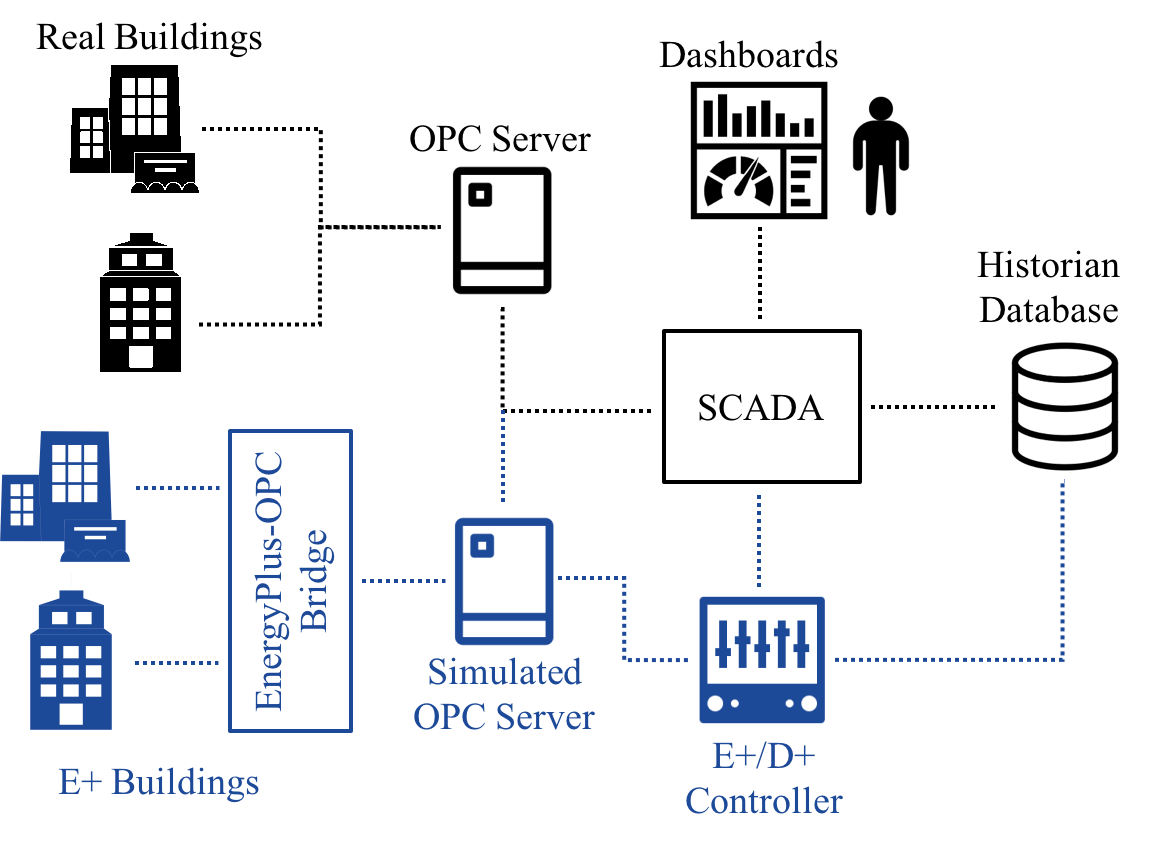
\includegraphics[width=0.5\textwidth]{images/overview.png}
	\caption{A typical architecture of a SCADA system working with a real building is shown in black, and our contributions in blue. We use an EnergyPlus OPC bridge that connects E+ models to the SCADA system through a simulated OPC server. We design a predictive controller using D+ models learned from the historical data obtained from a Historian database. For testing the controller with E+ models, the controller communicates via the OPC server. For testing the controller on a real building, secure and direct communication with SCADA is possible.}
	\label{F:intro}
\end{figure}